\documentclass[10pt,twocolumn,letterpaper]{article}

\usepackage{cvpr}
\usepackage{times}
\usepackage{epsfig}
\usepackage{graphicx}
\usepackage{amsmath}
\usepackage{amssymb}
\usepackage{mathrsfs}
\usepackage{mathtools}
\usepackage{subfigure}
\usepackage{pbox}
\DeclareMathOperator*{\argmin}{arg\,min}
% Include other packages here, before hyperref.

% If you comment hyperref and then uncomment it, you should delete
% egpaper.aux before re-running latex.  (Or just hit 'q' on the first latex
% run, let it finish, and you should be clear).
\usepackage[pagebackref=true,breaklinks=true,letterpaper=true,colorlinks,bookmarks=false]{hyperref}

\newcommand{\deva}[1]{\textcolor{red}{[Deva: #1]}}
\newcommand{\songfan}[1]{\textcolor{blue}{[Songfan: #1]}}

% \cvprfinalcopy % *** Uncomment this line for the final submission

\def\cvprPaperID{1627} % *** Enter the CVPR Paper ID here
\def\httilde{\mbox{\tt\raisebox{-.5ex}{\symbol{126}}}}

% Pages are numbered in submission mode, and unnumbered in camera-ready
\ifcvprfinal\pagestyle{empty}\fi
\begin{document}

%%%%%%%%% TITLE
\title{Supplementary Material for ``DAG-CNNs for multi-scale recognition''}

\author{First Author\\
Institution1\\
Institution1 address\\
{\tt\small firstauthor@i1.org}
% For a paper whose authors are all at the same institution,
% omit the following lines up until the closing ``}''.
% Additional authors and addresses can be added with ``\and'',
% just like the second author.
% To save space, use either the email address or home page, not both
\and
Second Author\\
Institution2\\
First line of institution2 address\\
{\tt\small secondauthor@i2.org}
}

\maketitle
%\thispagestyle{empty}

%%%%%%%%% ABSTRACT
%\begin{abstract}
%We explore multi-scale convolutional neural nets (CNNs) for image classification. Contemporary approaches extract features from a single output layer. By extracting features from multiple layers, one can simultaneously reason about high, mid, and low-level features during classification. The resulting multi-scale architecture can itself be seen as a feed-forward model that is structured as a directed acyclic graph (DAG). We show that DAG-CNNs are just as fast as chain-structured CNNs in terms of training and testing. In fact, training is easier because multi-scale connections tend to minimize the vanishing gradient problem. We present extensive analysis and results on standard scene benchmarks and show state-of-the-art classification performance on all benchmarks, \ie 55.5\% on SUN397, 76.1\% on MIT67, and 92.4\% on Scene15.
%
%\end{abstract}

%%%%%%%%% BODY TEXT
We include additional details and diagnostic experiments on feature dimensionality, the effect of marginalization, and fine-tuning.

\section{Feature dimension}
Most existing methods that use CNNs as feature extractors work with the last layer (or the last fully connected layer), yeilding a feature vector of size 4096. Our multi-scale model generates a feature vector of size 9216, {\em making it a factor of 2 larger} and so quite easy to use in practice.

{\bf Details:} We provide the exact breakdown of feature dimensionality for our Caffe-DAG model. Our forward selection from  Fig. 7(a) (of the main paper) chooses 5 RelU layers, whos dimensionalities are given in Table.~\ref{table:feat_dim}.

\begin{table}[htbp]
\begin{center}
\begin{tabular}{|c|c|c|c|}
\hline
Layer & Response &  Full Feat.& Marginal Feat.\\
\hline
11 & $13\times 13 \times 384$ & 64896 & 384 \\
13 & $13\times 13 \times 384$ & 64896 & 384 \\
15 & $13\times 13 \times 256$ & 43264 & 256 \\
18 & $1\times 1 \times 4096$ & 4096 & 4096 \\
20 & $1\times 1 \times 4096$ & 4096 & 4096 \\
\hline
Total& & 181248 & 9216\\
\hline
\end{tabular}
\end{center}
\caption{Feature Dimension for Caffe-DAG}
\label{table:feat_dim}
\end{table}



{\bf Full vs Marginal Features:} The above table suggests that it is crucial to use marginal features to keep the final dimensionality of the multi-scale feature manageable. A reasonable question is whether some performance is sacrificed for this reduced dimensionality. To evaluate this hypothesis, we build on the single-scale diagnostic experiments from our paper (Fig 3). Recall these experiments train and test an SVM on activations from a single-layer. We repeat these experiments using both full and marginal activation features each layer. For simplicity, we focus on 5 layers selected through forward selection (Table~\ref{table:perf_full}).

%We then train 67-way one-vs-all linear SVM classifiers similar to the experimental setups in the Section 4 for each layer. The classification accuracy is reported in Table.~\ref{table:perf_full}. The performances are identical for Layer-18 and Layer-20 since the \textit{Full-} and \textit{Marginal-feature} are equivalent. Surprisingly, as seen from Table.~\ref{table:perf_full}, the marginal-features always out-perform the full-feature for Layer-11, Layer-13, and Layer-20. This suggests that the full-features is likely to suffer from the ``curse of dimensionality'' given fairly small amount of training data (approximately 5k for MIT67). Thus, choosing marginal over full feature not only improves the classification performance but also reduces feature dimension to manageable ranges. 

\begin{table}[htbp]
\begin{center}
\begin{tabular}{|l|c|c|}
\hline
Layer & Full Feat. & Marginal Feat. \\
\hline
11 & 46.7 & 49.3  \\
13 & 49.0 & 53.8  \\
15 & 52.2 & 54.0  \\
18 & 60.2 & 60.2  \\
20 & 59.6 & 59.6  \\

\hline
\end{tabular}
\end{center}
\caption{Single-scale classification accuracy (\%) of Full vs. Marginal Features. \deva{If we have time, perhaps show as a bar plot?}}
\label{table:perf_full}
\end{table}

 Perhaps suprisingly, we find that {\em marginal features always outperform the full dimensional feature}, implying that dimensinality reduction actually helps performance. We verified that this phenomena was due to overfitting; the full features always performed better on training data, but performed worse on test data. This suggests that with additional training data, the full-dimensionality features may perform better.

\section{Model fine-tuning}

In this section, we further analyze ``off-the-shelf'' and ``fine-tuned'' versions of our multi-scale DAG model. Off-the-shelf models use multi-scale features extracted from pre-trained CNN (e.g., trained on ImageNet). Fine-tuned models retrain the entire DAG, in an end-to-end fashion, on the target dataset. For these experiments, our target dataset is MIT 67. 
%we take a deep-dive and consider training our DAG-CNN model in the end-to-end fashion. Firstly, we compare training the Chain and DAG models with softmax loss. We term them \textit{fine-tune} models. Secondly, we use the fine-tune model for feature extraction and analyze the performance of single- and multi-scale fine-tune models. All the experiments in this section is conducted on MIT67. 

\begin{table}[htbp]
\begin{center}
\begin{tabular}{|l|c|}
\hline
Structure & Accuracy \\
\hline
Off-the-shelf Caffe-Chain & 59.6   \\
Fine-tuned Caffe-Chain & 61.7 \\
Fine-tuned Caffe-DAG & 63.5\\
\hline
\end{tabular}
\end{center}
\caption{The comparison of fine-tune Models on MIT67. \deva{If we have time, perhaps show as a bar plot?}}
\label{table:ft_models}
\end{table}

{\bf Fine-tuned DAG:} We train a multi-scale DAG-CNN by iterative fine-tuning, making use of a sequence of pre-trained models. We tabulate the results in Table~\ref{table:ft_models}. We begin with off-the-shelf Caffe model. Using a single output layer (as is standard practice) yeilds a classification accuracy of 59.6\%. Next, we use this model to initialize gradient-based ``fine-tuning'', using training data from MIT-67. This produces a small improvement to 61.7\%. We plot the training and testing accuracy during training epochs in Fig.~\ref{fig:ft_curve}-(a). Finally, we use this fine-tuned chain model to initialize gradient-based learning of a DAG-CNN. To do so, we add multi-scale connections to the chain-structured ``backbone'', as shown in Fig 8 (main paper). The multi-scale weights are initialized to 0, while all other weights in the model are left as-is. End-to-end fine-tuning of our DAG noticeably improves accuracy to 63.5\%. We plot training and testing accuracy during training epochs in Fig.~\ref{fig:ft_curve}-(b). These experiments validate our end-to-end multi-scale training.

{\bf Off-the-shelf vs fine-tuned DAG:} However, an off-the-shelf DAG performs just as well (or even marginally better than) our fine-tuned DAG. As listed in our main paper, an off-the-shelf DAG produces an accuracy of 64.6. This suggests that while single-scale features don't transfer that well (from ImageNet to MIT67), multi-scale features transfer quite well between the two datasets. In fact, {\em multi-scale features transfer so well that no fine-tuning is apparently needed}. This validates our original hypotheses: multi-scale features are important for learning a generic feature extractor.%, that is applicable to a wide variety of recognition problems (that require both coarse and fine spatial reasoning).




%\subsection{Chain vs. DAG} 

%We use the generalized back-propagation algorithm presented in Section 3 to ``fine-tune'' the \textit{DAG} model on MIT67. In comparison, the traditional \textit{Chain} model is also fine-tuned in the same fashion. The data pre-processing step is the same as the one described in Section 4. To prevent over-fitting~\cite{AlexNet}, a dropout layer is inserted after the last FC layer, with the dropout rate of 0.5. The fine-tune chain model is initialized with the pre-trained Caffe model on ImageNet. As we can see from Fig.~\ref{fig:ft_chain}, the final accuracy saturates at 60.7\%. We then initialized our DAG model training with the fine-tuned chain model. As seen from the learning curve shown in Fig.~\ref{fig:ft_dag}, the DAG model stimulates the saturated Chain model and continues to drive the classification performance. Overall, the Caffe-DAG model out-performs the Caffe-Chain, as seen in Table.~\ref{table:ft_models}.


\begin{figure}
\centering
	\subfigure[Chain]{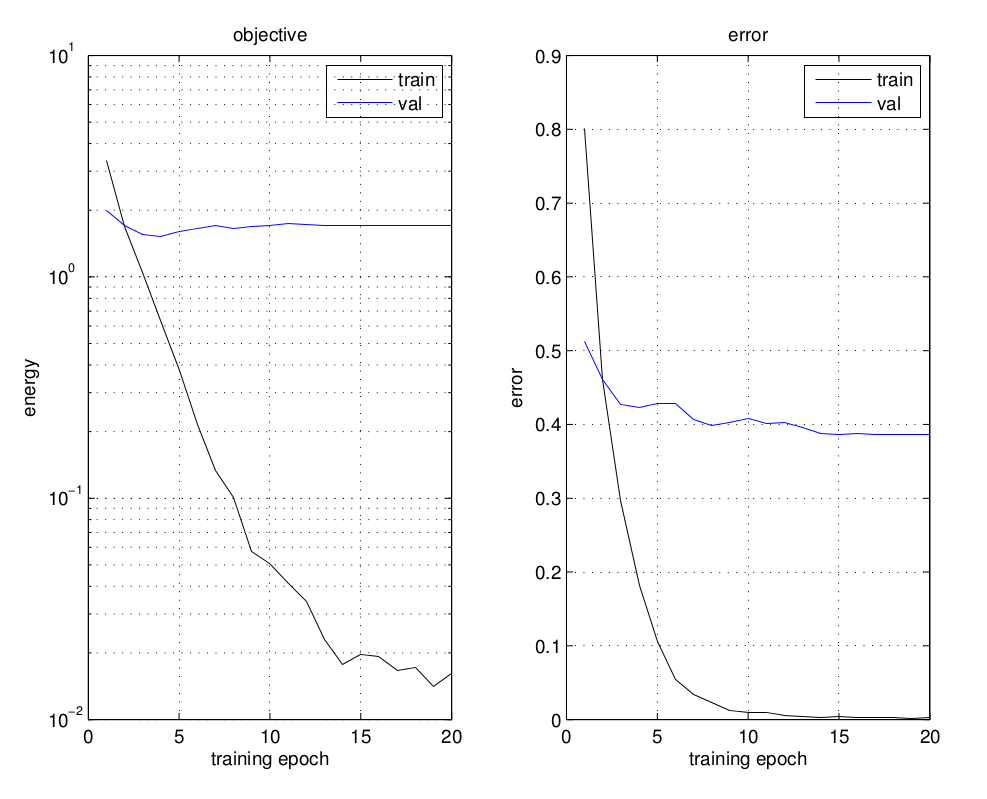
\includegraphics[width=.9\columnwidth]{fig/ft_chain.png}\label{fig:ft_chain}}
	\subfigure[DAG]{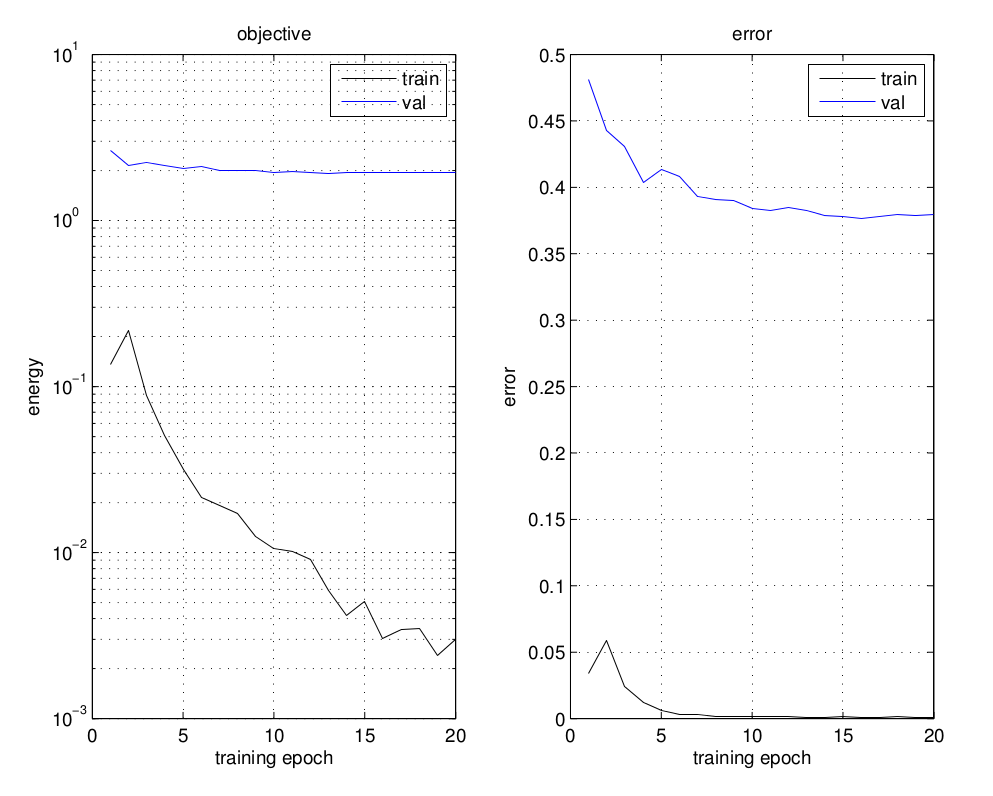
\includegraphics[width=.9\columnwidth]{fig/ft_DAG.png}\label{fig:ft_dag}}

\caption{Fine-tuning Caffe models on MIT67. The left shows the objectives for training and validation set for each epoch; the right shows the corresponding top-1/top-5 training and validation error. \deva{If we have time, remove top-5 from plot.}}
\label{fig:ft_curve}
\end{figure}


%\subsection{Fine-tuning vs. Off-the-shelf} 

%In the following experiment, we intend to understand the performance when fine-tune model is used for feature extraction. We compare three variants in this analysis, namely, \textit{off-the-shelf DAG}, \textit{fine-tune-chain DAG}, and \textit{fine-tune DAG}. The \textit{off-the-shelf DAG} is a special case of the multi-scale DAG model, as described in Section 3 of the main paper. It uses the Caffe backbone pre-trained with ImageNet dataset. Its features are extracted such that the ReLU activations are first average-pooled and l2-normalized. The multi-layer feature is by concatenating all single-layer features. The feature extraction for \textit{fine-tune-chain DAG} model follows the same procedure as off-the-shelf DAG; the only difference is we fine-tune the chain backbone on MIT67. As far as the \textit{fine-tune DAG} is concerned, we uses the generalized back-propagation to train the entire DAG model on MIT67. The activation of each average-pool layer is then extracted as feature, which can be visualized in Fig. 8 in the main paper. 

%Similar to all experiments on MIT67, 67-way one-vs-all classifiers are trained. The classification accuracy for all three settings are reported in Table.~\ref{table:ft_ots}. Firstly, we observe that multi-scale features always out-performs the best single-scale feature in all three cases. Secondly, the fine-tune models have superior performance for high-level features and the opposite for mid-level features. This suggests that fine-tuning tend to focus on improving the discriminativeness of high-level features. When combining multi-scale features, the off-the-shelf DAG has the largest performance boost due to the superior performance of mid-level features. Overall, the DAG models enjoy a consistent performance improvement by incorporating multi-scale features. 


%\begin{table}[htbp]
%\begin{center}
%\begin{tabular}{|l|c|c|c|c|c|c|}
%\hline
% & L11 & L13 & L15 & L18 & L20 & multi \\
%\hline
%off-the-shelf & \textbf{49.3} & \textbf{53.8} & 54.0 & 60.2 & 59.6 & \textbf{64.6} \\
%fine-tune-chain & 48.4 & 51.0 & 55.1 & 61.3 & \textbf{61.7} & 63.5 \\
%fine-tune   & 47.8 & 51.6 & \textbf{55.7} & \textbf{61.6} & 61.0 & 63.2	\\
%\hline
%\end{tabular}
%\end{center}
%\caption{Single- / Multi-scale feature performance for three variants of the DAG models on MIT67}
%\label{table:ft_ots}
%\end{table}



%
%\section{Fine-tune vs. Off-the-shelf}
%
%In this section, we analyze the performance of DAG-CNN trained in the end-to-end fashion on all three datasets. These results is then compared with the off-the-shelf DAG-CNN feature. Concretely, we first train the proposed DAG-CNN model with softmax loss using the algorithm presented in Section 3. We term this \textit{fine-tune} model. On the other hand, the \textit{off-the-shelf} setting is by first concatenating the outputs of the average-pooled features and then trained with hinge loss using Liblinear package~\cite{liblinear}. The results for \textit{off-the-shelf} experimental setup are the reported in the main paper. Here, we provide the results for the \textit{fine-tune} setup as a comparison. 
%
%
%\begin{table}[htbp]
%\begin{center}
%\begin{tabular}{|l|c|c|}
%\hline
%Approach & Off-the-shelf &  Fine-tune\\
%\hline
%Deep19-DAG & \textbf{55.5} &  \\
%Deep19~\cite{veryDeep} & 51.9 &  \\
%Caffe-DAG & 46.6	& \\
%Caffe~\cite{Caffe} & 43.5 &  \\ \hline
%
%\hline
%\end{tabular}
%\end{center}
%\caption{Classification results on SUN397}
%\label{table:SUN397}
%\end{table}
%
%
%
%\begin{table}[htbp]
%\begin{center}
%\begin{tabular}{|l|c|c|}
%\hline
%Approach & Off-the-shelf &  Fine-tune\\
%\hline
%Deep19-DAG & \textbf{76.1} &  \\
%Deep19~\cite{veryDeep} & 70.8 &  \\
%Caffe-DAG & 64.6	& 63.5\\
%Caffe~\cite{Caffe} & 59.5 & 60.7 \\ \hline
%
%\hline
%\end{tabular}
%\end{center}
%\caption{Classification results on MIT67}
%\label{table:MIT67}
%\end{table}
%
%
%
%\begin{table}[htbp]
%\begin{center}
%\begin{tabular}{|l|c|c|}
%\hline
%Approach & Off-the-shelf &  Fine-tune\\
%\hline
%Deep19-DAG & \textbf{92.4} &  \\
%Deep19~\cite{veryDeep} & 90.8 &  \\
%Caffe-DAG & 89.7	& \\
%Caffe~\cite{Caffe} & 86.8 & \\ \hline
%
%\hline
%\end{tabular}
%\end{center}
%\caption{Classification results on Scene15}
%\label{table:Scene15}
%\end{table}



{\small
\bibliographystyle{ieee}
\bibliography{mobib}
}

\end{document}
